\section{\emph{Resource Description Framework}}
\emph{Resource Description Framewok (RDF)} merupakan dasar pembentuk basis pengetahuan dalam semantik web, diajukan oleh W3C sebagai standar pada tahun 1999. RDF terdiri dari subjek, predikat dan objek yang kemudian dikenal dengan naman \emph{statement}. Subjek dapat berupa URI (Uniform Resource Identifier) yang berfungsi sebagai penanda atau \emph{identifier}, tidak menuntup kemungkinan sebuah subjek juga dapat berupa URL \emph{(Uniform Resource Locator)} yang merupakan bentuk khusus dari URI.  Predikat berupa URI yang menjelaskan hubungan antara subjek dengan objeknya sedangkan objek dapat berupa URI ataupun \emph{literal}. Sebuah pernyataan dalam RDF disebut dengan istilah \emph{triple}. secara grafis, bentuk \emph{statement} RDF dapat dilihat pada gambar \ref{fig:rdf_statement}.

\begin{figure}[ht]
	\centering
	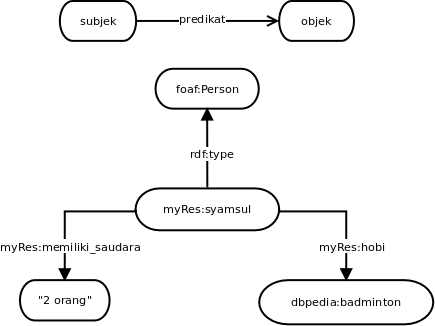
\includegraphics[trim = 29mm 141mm 40mm 0mm, clip, scale=0.6]{gambar}
	\caption{Struktur \emph{statement} RDF}
	\label{fig:rdf_statement}
\end{figure}

Sebagai contoh misalnya pernyataan ``Syamsul hobi badminton'', ``Syamsul memiliki saudara 2 orang'', pernyataan-pernyataan tersebut dapat dibentuk menjadi sebuah \emph{triple}. Pada pernyataan pertama, \emph{Syamsul} adalah merupakan subjek sedangkan \emph{hobi} merupakan sebuah predikat dan \emph{badminton} merupakan sebuah objek, sedangkan pada pernyataan kedua yang menjadi subjek adalah \emph{Syamsul} sedangkan predikat adalah \emph{memmiliki saudara} dan \emph{2 orang} merupakan objek. Jika objek pada pernyataan pertama di atas memerlukan penjelasan lebih lanjut, misalnya mengenai apa itu badminton, maka objek tersebut dapat berupa \emph{resource} dimana \emph{resource} tersebut membentuk triple-triple seperti terlihat pada gambar \ref{fig:rdf_multi_statement}. Pada pernyataan kedua, hanya dimungkinkan berupa literal karena tidak memerlukan penjelasan lebih lanjut mengenai objek itu sendiri.

Agar dapat di proses oleh komputer maka RDF triple harus dituliskan dalam bahasa atau sintak yang dapat dimengerti oleh komputer. Hingga saat ini bentuk penulisan RDF yang direkomendasikan oleh W3C adalah dalam bentuk XML dengan menggunakan namespace yang khusus RDF. Contoh statement di atas dapat kita serialisasi menjadi RDF sebagai berikut:
\lstinputlisting[firstline=1, lastline=7]{./parts/codeblock.xml}
\begin{figure}[ht]
	\centering
	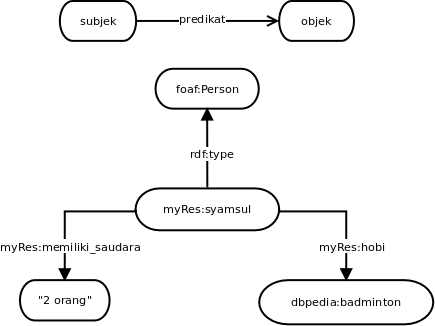
\includegraphics[trim = 0mm 0mm 0mm 93mm, clip, scale=0.55]{gambar}
	\caption{RDF dengan multi-statement}
	\label{fig:rdf_multi_statement}
\end{figure}
Selain XML/RDF, RDF juga dapat dituliskan dengan menggunakan Turtle sintaks sebagai berikut:
\lstinputlisting[firstline=9, lastline=11]{./parts/codeblock.xml}

Sintaks turtle lebih mudah dipahami oleh manusia, sehingga lebih mudah dibentuk. Meskipun sintak ini masih belum menjadi rekomendasi W3C namun besar kemungkinan kedepan juga akan menjadi rekomendasi karena sudah memiliki draft yang dapat dilihat di http://www.w3.org/TR/turtle/.